\begin{frame}{Inference refs}
%\printbibliography[keyword={inference}]
\end{frame}

\section{Likelihood and degree of belief}

\begin{frame}{Funzione di Likelihood}
\begin{block}{Funzione di likelihood}
\begin{columns}[T]
\begin{column}{0.5\textwidth}
\[L_{x_0}(m)=p(x_0;m)\]
x,y: eventi indipendenti:
\[L_{(x_0,y_0)}(m)=L_{x_0}(m)L_{y_0}(m)\]
\end{column}
\begin{column}{0.5\textwidth}
Definita a meno di costante moltiplicativa ($\log{L}$): invariante per cambiamento di osservabile (funzione solo dei dati)
\[L_{f(t_0)}(m)=|J(t_0)|L_{t_0}(m)\]
\end{column}
\end{columns}
\end{block}
\begin{columns}[T]
\begin{column}{0.5\textwidth}
\begin{block}{T di Bayes e likelihood}
Se posso definire una $p(\theta)$:
\begin{align*}
&p(\theta|x_0)=\frac{p(x_0|\theta)p(\theta)}{p(x_0)}\\
&\posterior{}=\frac{\likelihood{}\prior{}}{\int p(x_0|\theta)p(\theta)\,d\theta}
\end{align*}
\end{block}
\end{column}
\begin{column}{0.5\textwidth}
\begin{block}{Degree of belief}
Posterior ratio: $\frac{\Pi(\theta_1|x_0)}{\Pi(\theta_2|x_0)}=\frac{L_{x_0}(\theta_2)}{L_{x_0}(\theta_1)}\frac{\Pi(\theta_2)}{\Pi(\theta_1)}$.
\end{block}
\end{column}
\end{columns}
\begin{block}{Metodo di massima likelihood}
Ripetendo gli esperimenti la likelihood diventa pi\'u piccata.
\end{block}
\end{frame}

\begin{frame}{Esempi di Likelihood: uniforme, bernoulli, ...}
\begin{block}{Likelihood per distro uniforme}
\pgfmathsetmacro{\unifM}{3}
\begin{columns}[T]
\begin{column}{0.5\textwidth}
\begin{tikzpicture}[scale=0.5,domain=0:1.5*\unifM]
\pgfmathsetmacro{\unifN}{(\unifM)^-1}
\begin{axis}[ylabel={$p(x;m)$},extra x ticks={\unifM}, extra x tick labels={$m$},
        extra x tick style={xticklabel style={yshift=-10}}]
%\draw[->] (-0.2,0) -- (1.5*\unifM,0) node[right] {$x$};
%\draw[->] (0,-0.2) -- (0,1.5*\unifM) node[above,red] {$p(x;m)$};
%\draw[color=red] plot[domain=0:\unifM, id=unif] function{\unifN} node[right] {$\frac{1}{m}$};
    \addplot[color=red] function [raw gnuplot, id=unifpdf, mark=none]{set xrange [0:\unifM]; plot \unifN};
\end{axis}
\end{tikzpicture}
\end{column}
\begin{column}{0.5\textwidth}
\begin{tikzpicture}[scale=0.5]
\begin{axis}[ylabel={$\mathcal{L}_{x_0}(m)$},extra x ticks={\data},extra x tick labels={$x_0$},
        extra x tick style={xticklabel style={yshift=-10}}]
\pgfmathsetmacro{\data}{(rand+1)/2*\unifM}
\pgfmathsetmacro{\unifN}{(\unifM)^-1}
    \addplot[color=orange] function [raw gnuplot, id=unifL, mark=none]{set xrange [\data:*]; plot 1/x};
\end{axis}
\end{tikzpicture}
\end{column}
\end{columns}
\end{block}
\begin{columns}[T]
\begin{column}{0.5\textwidth}
    \begin{block}{Likelihood per distro uniforme}
\begin{align*}
&L_0=1-p\\
&L_1=p
\end{align*}
\end{block}
\end{column}
\begin{column}{0.5\textwidth}
\begin{block}{Likelihood di pi\'u misure e statistiche}
\begin{align*}
&\prob{(t,\tau)}=\frac{1}{\tau}\exp{-\frac{t}{\tau}}\\
&L_{(t_1,\ldots,t_n)}(\tau)=\prod_i^n\frac{1}{\tau}\exp{-\frac{t_i}{\tau}}\\
&=\frac{1}{\tau^n}\exp{-\frac{\sum t_i}{\tau}}=\frac{1}{\tau^n}\exp{-\frac{n\overline{t}}{\tau}}
\end{align*}
\end{block}
\end{column}
\end{columns}
\end{frame}

\begin{frame}{Esercizi su Likelihood applicata}
\keyword{Ex: likelihood pdf exp; decadimento in volo particella.}
Distribuzione esponenziale in x: quale z?
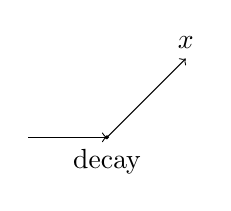
\begin{tikzpicture}
\draw[->] (0,0)--(1,0) node[draw,fill,circle,minimum size=1pt,inner sep=0,label=below:decay] {};
\draw[->] (1,0)--(2,1) node[above] {$x$};
\end{tikzpicture}
\end{frame}

\begin{frame}{Statistiche sufficienti per il parametro dato}
\begin{block}{Statistica sufficiente $S$}
Pdf di X data $S(X)$ non dipende da parametro $\theta$
\begin{columns}[T]
\begin{column}{0.5\textwidth}
Probabilit\'a di osservare $x$ in funzione di $\theta$ \'e probabilit\'a di $S(x)$ dato $\theta$ per funzione sole osservabili: \[\prob{(x;\theta)}=\prob{(S(x);\theta)}h(x)\] e $\omega_{\theta}$ non dipende da $\theta$.
\end{column}
\begin{column}{0.5\textwidth}
pdf di $X$ dato $T(X)$ non dipende da $\theta$:
\[\prob{(x;S,\theta)}=\prob{(x;S)}\]
\end{column}
\end{columns}
\end{block}
\begin{block}{Statistica sufficiente minimale}
$S$ sufficiente e esiste una funzione $f$ per ogni $s_i$ con $S=f(s_i)$ e $\dim({S})\leq\dim{(X)}$.
\end{block}
\begin{block}{Teorema di Darmois: condizione necessaria e sufficiente}
Esiste S tale che $\dim{(S)}<\dim{(X)}$ iff
\begin{align*}
&p(\vec{x}|\theta)=\Exp{[\sum_i^n\alpha_i(\vec{x})a_i(\theta)+\beta(\vec{x})+\gamma(\theta)}\ \text{\keyword{famiglia esponenziale}}\\
&S_i=\sum_j\alpha_i(x_j)
\end{align*}
\end{block}
\end{frame}

\begin{wordonframe}{Statistiche sufficienti: esempi.}
$\vec{x}=\{x_1,\ldots,x_n\}$: $T(\vec{x})$ sufficiente iff $L(T,\theta)=g(T,\theta)h(\vec{x})$ e dominio $\omega_{\theta}$ non dipende da $\theta$.
\begin{align*}
&L(x;\mu,\sigma)=\frac{1}{\sqrt{2\pi}\sigma}\exp{-\frac{1}{2}\frac{(x-\mu)^2}{\sigma^2}}\\
&\overline{x}=\frac{\sum x_i}{N}:\ L(\overline{x};\mu)=\prod_iL(x_i;\mu,\sigma)=(\frac{1}{\sqrt{2\pi}\sigma})^N\exp{-\frac{1}{2}\frac{\sum_i(x_i-\mu)^2}{\sigma^2}}
\end{align*}
\begin{block}{Gaussiana: media ignota, varianza nota}
\begin{align*}
&L(\overline{x};\mu)=\prod_iL(x_i;\mu,\sigma)=(\frac{1}{\sqrt{2\pi}\sigma})^N\underbrace{\exp{-\frac{N}{2}\frac{\sum_i(\overline{x}-\mu)^2}{\sigma^2}}}_{g(T,\theta)}\underbrace{\exp{-\frac{N}{2}\frac{\sum_i(x_i-\overline{x})^2}{\sigma^2}}}_{h(\vec{x}}
\end{align*}
La statistica ''media aritmetica'' \'e sufficiente per parametro $\mu$ della gaussiana (dominio gaussiana non dipende da $\mu$) (\keyword{Ex: pdf della media aritmetica})
\end{block}
\begin{block}{Gaussiana: media nota, varianza ignota}
$\hat{\sigma}^2=\frac{\sum x_i^2-\mu}{N}$ \'e sufficiente per $\sigma^2$ (pdf di $\hat{\sigma}^2\propto g$ e dominio gaussiana non dipende da $\sigma$). (\keyword{Ex: statistica sufficiente $\sigma$ gaussiana})
\end{block}
\begin{block}{\keyword{Media aritmetica \'e statistica sufficiente per parametro binomiale, poissoniana, esponenziale }}
\begin{align*}
&\prob{(k)}=\binom{n}{k}p^k(1-p)^{n-k}\\
&\prob{(k)}=\frac{\mu^k\exp{-\mu}}{k!}\\
&\prob{(x)}=\lambda\exp{-\lambda x}
\end{align*}
\end{block}
\begin{block}{Distribuzione uniforme: statistica $x_{max}$}
\begin{columns}[T]
\begin{column}{0.5\textwidth}
\pgfmathsetmacro{\unifM}{3}
\begin{tikzpicture}[scale=0.5,domain=0:1.5*\unifM]
\pgfmathsetmacro{\unifN}{(\unifM)^-1}
\begin{axis}[ylabel={$p(x;m)$},extra x ticks={\unifM}, extra x tick labels={$m$},
        extra x tick style={xticklabel style={yshift=-10}}]
%\draw[->] (-0.2,0) -- (1.5*\unifM,0) node[right] {$x$};
%\draw[->] (0,-0.2) -- (0,1.5*\unifM) node[above,red] {$p(x;m)$};
%\draw[color=red] plot[domain=0:\unifM, id=unif] function{\unifN} node[right] {$\frac{1}{m}$};
    \addplot[color=red] function [raw gnuplot, id=unifpdf, mark=none]{set xrange [0:\unifM]; plot \unifN};
\end{axis}
\end{tikzpicture}

\end{column}
\begin{column}{0.5\textwidth}
\begin{align*}
&\prob{(x;m)}=\left\{\begin{matrix}\frac{1}{m}\ x\in[0,m]\\0\\\end{matrix}\right.&\intertext{estraggo N $x_1,\ldots,x_n$}\\
&L(\vec{x},m)=\prod_iL(x_i;m)=\left\{\begin{matrix}\frac{1}{m^N}\ m>x_{max}\\0\ m<x_{max}\\\end{matrix}\right.
\end{align*}
\end{column}
\end{columns}
$g(T,\theta)\propto A(T;\theta)$ dove $A$ \'e pdf di statistica $T$?
\begin{align*}
&\prob{(x_{max}<x_0)}=F_M(x_0)=\prod_i\prob{(x_i<x_0)}=\prod_i\int_0^{x_0}\frac{1}{m}\,dx=(\frac{x_0}{m})^N\\
&\prob{(x_M;m)}=\TDof{x_0}\left.F_M(x_0)\right|_{x_M}=\frac{N}{m}(\frac{x_M}{m})^{N-1}\\
&L_{\vec{x}}(m)=\frac{N}{m^N}x_M^{N-1}\frac{1}{Nx_M^{N-1}}=\prob{(x_M;m)}\frac{1}{Nx_M^{N-1}}\ m>x_M
\end{align*}
\end{block}
\keyword{Ex: Per pdf uniforme $x_{min}$ \'e sufficiente per m?}
\end{wordonframe}

\begin{wordonframe}{Applicazioni T Darmois}
\begin{block}{Poisson}
\begin{align*}
&\frac{\exp{-\mu}\mu^k}{k!}=\exp{\mu}\exp{k\ln{\mu}}\exp{-\ln{k!}}\\
&S=\sum_i^Nk_i
\end{align*}
\end{block}
\keyword{Ex: Come procedo se pdf non esponenziale (LHC)?}
\end{wordonframe}

\section{Inferenza statistica. Paradigma frequentista e bayesiano.}
%\begin{refsection}{}
\subsection{Principio di sufficienza}

\begin{frame}{Principio di sufficienza}
\begin{block}{Principio di sufficienza}
Sia $E$ un esperimento con spazio campionario definito da $X$ e $S(X)$ una statistica sufficiente; sia $E'$ l'esperimento derivato con stesso spazio spazio dei parametri e tale che quando in $E$ \'e osservato x in $E'$ \'e osservato $t=t(x)$.
Principio di sufficienza: per ogni x $Ev(E,x)=Ev(E',t)$.
\end{block}
\begin{block}{Principio di likelihood (Fisher Barnard)}
    Se osservo x tutta informazione statistica in $L_x$: $L_x=L_y$ allora stesse inferenze da x e y. (Se $E$ e $E'$ hanno stesso spazio dei parametri e $x$, $y$ sono due misure le cui likelihood soddisfano $f(x,\theta)=cg(y,\theta)$ per ogni $\theta$ allora $Ev(E,x)=Ev(E',y)$
\end{block}
\end{frame}

\subsection{Principio di condizionalit\'a}

\subsection{Paradigmi di inferenza}

\begin{frame}{Paradigmi}
\begin{block}{Fisher}

\end{block}
\begin{block}{Neyman Pearson}

\end{block}
\begin{block}{Bayesian}
Il teorema di Bayes \'e usato per aggiornare la probabilit\'a sulla base di nuove informazioni. 
\end{block}
\end{frame}

\subsection{Baysiano}

\subsection{Informazione}

\begin{frame}{Informazione di Fischer}
Informazione contenuta nei dati su un parametro $\Theta$
\begin{align*}
&I_X(\Theta)=\E_{\Theta}{[(\PDof{\Theta}\log{f(X;\Theta}))^2]}=-\E_{\Theta}{[\PtwoDof{\Theta}\log{f(X;\Theta)}]}
\end{align*}
Per due parametri:
\begin{align*}
&I_X(\Theta)=\begin{pmatrix}I_{11}(\Theta)&I_{12}(\Theta)\\I_{21}(\Theta)&I_{22}(\Theta)\end{pmatrix}\ I_{ij}(\Theta)=-\E{[\frac{\partial^2}{\partial\Theta_i\partial\Theta_j}\log{f(X;\Theta)}]}
\end{align*}
\begin{block}{Informazione e statistiche}
$I_X(\Theta)\geq I_T(\Theta)$: l'uguaglianza vale iff T \'e sufficiente per $\Theta$.
\end{block}
\begin{align*}
&Y=h(X)\ 1-1 \Rightarrow I_X=I_Y\\
&X\to f(X;\Theta)\ Y\to g(Y;\Theta)=f(\invers{h}(Y);\Theta)|\TDy{y}{\invers{h}(Y)}|\\
&I_Y=\E_Y{[(\PDof{\Theta}\log{g(Y)})^2]}=\E_Y{[(\PDof{\Theta}\log{f(\invers{h}(Y)})^2]}\\
&=\E_X{[(\PDof{\Theta}\log{f(X)})^2]}
\end{align*}
\end{frame}

\begin{wordonframe}{Esempi Informazione}
\begin{columns}[T]
\begin{column}{0.33\textwidth}
\begin{block}{pdf Poisson}
\begin{align*}
&\log{f}=-\lambda\\
&+x\log{\lambda}-\log{x!}\\
&I_X(\lambda)=\invers{\lambda}
\end{align*}
\end{block}
\end{column}
\begin{column}{0.33\textwidth}
\begin{block}{pdf Gauss}
\begin{align*}
&\log{f}=-\frac{1}{2}\frac{(x-\mu)^2}{\sigma^2}\\
&-\log{(\sqrt{2\pi}\sigma)}\\
&I_X(\mu)=\sigma\expy{-2}
\end{align*}
\end{block}
\end{column}
\begin{column}{0.33\textwidth}
\begin{block}{n RV iid}
$X_1,\ldots,X_n$ n RV iid:
\begin{align*}
&X=\sum X_i\\
&I_X(\Theta)=nI_{X_1}(\Theta)
\end{align*}
\end{block}
\end{column}
\end{columns}
\begin{block}{n RV gaussiane $N(\mu,\sigma^2)$: matrice informazione}
$\vec{X}=(X_1,\ldots,X_n)$ e $\vec{\Theta}=(\mu,\sigma^2)$
\begin{align*}
&I_{11}=\E{[(\PDof{\mu}\log{f})^2]}=\sigma\expy{-2}\ I_{22}=\E{[(\PDof{\sigma^2}\log{f})^2]}=\frac{1}{2}\sigma\expy{-4}\\
&I_{12}=I_{21}=\frac{1}{2\sigma^2}\E{[\sigma\expy{-3}(X_1-\mu)^3-(X_1-\mu)]}=0
\end{align*}
\end{block}
\begin{block}{Perdita di informazione se tengo solo media campionaria delle RV gaussiane}
$\vec{X}=(X_1,\ldots,X_n)$ e media $\exv{X}=\frac{1}{n}\sum X_i$ con pdf $N(\mu,\invers{n}\sigma^2)=g(x,\Theta)=\frac{\sqrt{n}}{\sigma\sqrt{2\pi}}\exp{-\frac{n}{2\sigma^2}(x-\mu)^2}$
\begin{align*}
&I_{11}=\E{[(\PDof{\mu}\log{g})^2]}=n\sigma\expy{-2}\ I_{22}=\E{[(\PDof{\sigma^2}\log{g})^2]}=\frac{1}{2}\sigma\expy{-4}\\
&I_{12}=I_{21}=\frac{1}{2\sigma^2}\E{[\sigma\expy{-3}(X_1-\mu)^3-(X_1-\mu)]}=0\\
&I_{\vec{X}}-I_{\exv{X}}\geq0
\end{align*}
\end{block}
\begin{block}{Perdita di informazione se tengo solo la varianza campionaria delle RV gaussiane}
Varianza campionaria $S^2=\frac{1}{n-1}\sum_i(X_i-\exv{X})^2$ (\keyword{Gaussian variance: unbiased estimator}). 
La RV $Y=(n-1)\frac{S^2}{\sigma^2}$ ha pdf $\chi^2_{n-1}$: $c\exp{-\frac{1}{2}y}y\expy{\frac{n-3}{2}}$ con $c=2\expy{\frac{n-1}{2}}\Gamma(\frac{1}{2}(n-1))$
\begin{align*}
&S^2\to h(x;\theta)=d\sigma\expy{-(n-1)}\exp{-\frac{n-1}{2}\frac{x}{\sigma^2}}x\expy{\frac{n-3}{2}}\ d=c(n-1)^{\frac{n-1}{2}}\\
&I_{11}=I_{12}=I_{21}=0\ I_{22}=\frac{1}{2}(n-1)\sigma\expy{-4}:\\ &I_{\vec{x}}-I_{S^2}=\begin{pmatrix}n\sigma\expy{-2}&0\\0&\frac{1}{2}\sigma\expy{-4}\end{pmatrix}''\geq0''
\end{align*}
$\exv{X}$, $S^2$ are indipendently ($P(A\cap B)=P(A)P(B))$) distributed: $I_{\exv{X},S^2}=I_{\exv{X}}+I_{S^2}=I_{\vec{X}}(\Theta)$.
\end{block}
\end{wordonframe}

\begin{frame}{Come ridurre i dati se statistica sufficiente non \'e disponibili}
Perdita informazione
\begin{itemize}
\item istogramma
\item dati troncati
\end{itemize}
\end{frame}

\section{Stimatori}

\begin{frame}{Stimatori puntuali}
    
\end{frame}


%\end{refsection}
